% Author: Johannes Borgqvist
% Date: 2019-06-26
% Description: 
% Draws a system with an activator inhhibitor system with a positive 
% deedback loop
%------------------------------------------------------------------------
%The document
%------------------------------------------------------------------------
\documentclass[tikz, border=1pt]{standalone}
%------------------------------------------------------------------------
% Usepackages
%------------------------------------------------------------------------
\usepackage{verbatim}
%------------------------------------------------------------------------
% Libraries in tikz
%------------------------------------------------------------------------
\usetikzlibrary{arrows}
\usetikzlibrary{positioning}
%------------------------------------------------------------------------
% Setting up the document
%------------------------------------------------------------------------
\begin{document}
%------------------------------------------------------------------------
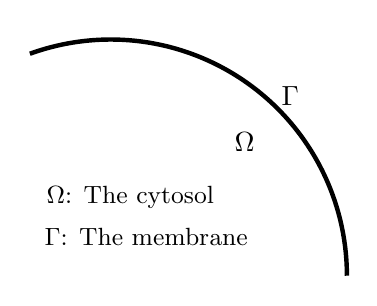
\begin{tikzpicture}
% Draw the membrane
%\filldraw[ultra thick,fill=brown,opacity=0.4]  (0.5,2.3) -- (0.5,2.98) (3,0) arc (0:90:3cm) (2.5,0) arc (0:90:2.5cm) (2.3,0.5) -- (2.95,0.5) ;
\draw[ultra thick] (3,0) arc (0:110:3cm);
% Give names to the various parts
\node at (1.7, 1.7)  (Cytosol)    {$\Omega$};
\node at (2.28, 2.28)  (Membrane)    {$\Gamma$};
% Explanations
\node[align=left] at (0.25, 1.0)  {\small$\Omega$: The cytosol};
\node[align=left] at (0.45, 0.5){\small$\Gamma$: The membrane};
% Figure Name
%\node at (-2.2, 4)    {\huge\textbf{(B)}};
\end{tikzpicture}
\end{document}
